\documentclass[a4paper,12pt]{article}

\usepackage{graphicx}   % For including images
\usepackage{setspace}   % For line spacing
\usepackage{geometry}   % To adjust margins
\usepackage{ragged2e}
\pagestyle{empty} % Remove page numbers
\geometry{margin=1in}   % Set margin size

\title{
  \vspace{-2em} % Adjust the space above the title
  \textbf{CS702- Computing Lab} \\ % Main title
  \large \textbf{ Department of Computer Science and Engg.- NITK Surathkal} \\ % Subtitle
  \vspace{1em} % Space between subtitle and author
  \textbf{ABHIJITH C} \\ % Author
  Roll Number: 242CS003 \\% Roll number
  \textbf{ANAND M K} \\ % Author
  Roll Number: 242CS008 \\% Roll number
}

\date{} % Remove the date

\begin{document}
\maketitle

% Title Page
\begin{titlepage}
\begin{center}

    \vspace*{0.1in}

    {\Huge\bfseries Pre-owned Car Price Prediction\par}
    \vspace{1in}
\end{center}

\section*{Introduction}
\begin{justify}

In today's world, where people’s living standards have greatly improved, cars have become a necessary part of life. The latest statistics show that the demand for used cars has increased significantly.  The average consumer may not have enough knowledge and information needed to accurately evaluate the price of a car they wish to buy, which can leave them vulnerable to being scammed. This is where price prediction using Machine Learning or Deep Learning becomes significant. This will give consumers a clear picture of current market prices and trends.  
\newline

The main goal of this project is to design a prediction model using the most accurate algorithm, which will be selected after comparing various Machine Learning and Deep Learning algorithms. The project also includes designing a user-friendly website that will enable consumers to use the prediction model to estimate prices effortlessly.
\newline

The motive of the project is to study and analyze various machine learning and deep learning algorithms, as well as to gain a clear understanding of different aspects of web development.

\end{justify}

\section*{Problem Statement and Objectives}
\begin{justify}

There are various parameters, such as mileage, kilometers driven, engine capacity, fuel type, etc., that must be considered to accurately predict prices. Therefore, it is challenging to calculate the price using traditional mathematical algorithms. Several Machine Learning regression algorithms, such as Linear Regression, Decision Tree, and Deep Learning, can be applied to these types of problems. However, identifying the best algorithm is a challenging task. The main objective of the project is to study, analyze, and compare these algorithms to build the most accurate model. The available data may contain duplicates and outliers, making it necessary to clean the data before using it to train the models. Another objective is to design a user-friendly, responsive, and fast-performing website that allows consumers to easily predict prices based on their requirements.

\end{justify}

\end{titlepage}

\newpage
\section*{Solution and Different Phases of the Project}
\begin{justify}
\begin{figure}[h]
    \centering
    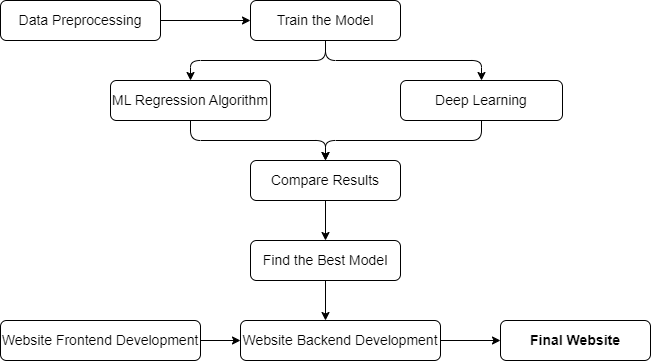
\includegraphics[width=.8\textwidth]{./projectflow1.png}
    \caption{Solution Flowchart}
    \label{fig:your-label}
\end{figure}
\vspace{\baselineskip} 
The first phase of the project is to find an appropriate dataset and perform data preprocessing. Datasets can be accessed from various websites, such as Kaggle. Python libraries, including Pandas and NumPy, can be used for this preprocessing. 
\newline

The second phase of the project is to train the model. The Scikit-learn library can be used for implementing machine learning regression algorithms, while TensorFlow and Keras can be used for training the dataset using neural networks.
\newline

The third phase of the project is to compare the performance of different algorithms using performance metrics such as Mean Absolute Error (MAE) and select the most accurate algorithm. This chosen algorithm will then be used to train the final model.
\newline

The fourth phase of the project is to develop the frontend of the website. This includes designing the UI, which will feature various input fields for parameters such as car model, year of registration, engine capacity, mileage, kilometers driven, etc. Additionally, there will be a "Predict" button that, when clicked, will process the inputs and present the results to the user. The designed UI can then be implemented using web development tools such as HTML, CSS, JavaScript, and React.js
\newline

The fifth phase of the project is to develop the backend of the website. This can be implemented using Python frameworks such as Flask or Django.
\newline

The sixth and final phase of the project involves integrating the frontend and backend through API calls. Following integration, testing will be conducted using various test cases. Finally, documentation for the project will be prepared.

\newpage
\section*{Exepected Outcomes}
	\begin{itemize}
		\item A predictive model that provides accurate predictions based on user inputs.
		\item A reliable and responsive website that accurately displays the expected price of a pre-owned car based on various input features.
		\item Successful integration of the frontend and backend.

	 \end{itemize}

\section*{Tentative Timeline}
\begin{figure}[h]
    \centering
    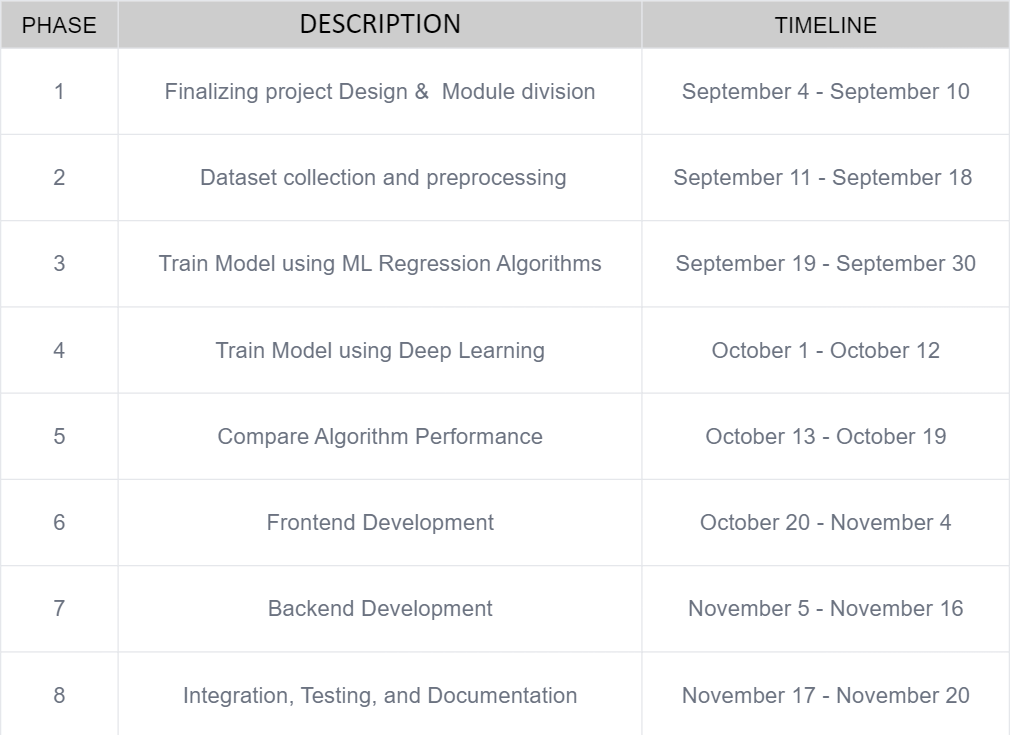
\includegraphics[width=.8\textwidth]{./timeline.png}
    \caption{Timeline}
    \label{fig:your-s}
\end{figure}


\begin{thebibliography}{9}
\bibitem{varshitha2022}
J. Varshitha, K. Jahnavi, and C. Lakshmi, "Prediction Of Used Car Prices Using Artificial Neural Networks And Machine Learning," \textit{2022 International Conference on Computer Communication and Informatics (ICCCI)}, Coimbatore, India, 2022, pp. 1-4, doi: 10.1109/ICCCI54379.2022.9740817.


\bibitem{kathiravan2023}
M. Kathiravan, M. Ramya, S. Jayanthi, V. V. Reddy, L. Ponguru, and N. Bharathiraja, "Predicting the Sale Price of Pre-Owned Vehicles with the Ensemble ML Model," \textit{2023 4th International Conference on Electronics and Sustainable Communication Systems (ICESC)}, Coimbatore, India, 2023, pp. 1793-1797, doi: 10.1109/ICESC57686.2023.10192988.


\end{thebibliography}

\end{justify}

\end{document}
